\documentclass[border=0pt]{standalone}
\usepackage{tikz,amssymb,url,amsmath,amsthm,listings,algorithm,algpseudocode,enumerate, caption, xspace, float, verbatim,tabularx,mathtools,adjustbox,pgfplots}
\usetikzlibrary{fit}
\usetikzlibrary{positioning}
\usetikzlibrary{math}
\usetikzlibrary{shapes.misc}
\usetikzlibrary{backgrounds}
\def\ba{{\boldsymbol a}}
\tikzset{cross/.style={cross out, draw=black, minimum size=2*(#1-\pgflinewidth), inner sep=0pt, outer sep=0pt},cross/.default={1pt}}
\begin{document}
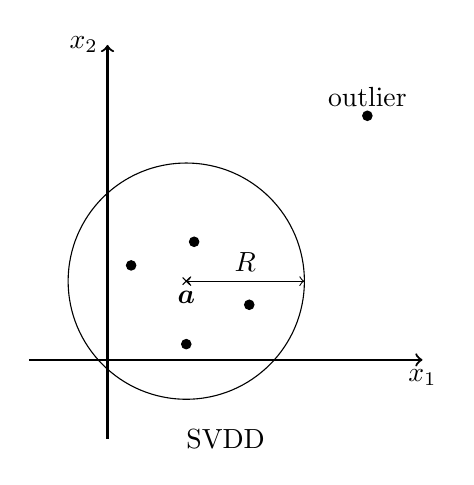
\begin{tikzpicture}[domain=-0.5:4,yscale=1,xscale=1,baseline,tight background]
	\tikzmath{\pax=1; \pay=0.2; \pbx=0.3; \pby=1.2; \pcx=1.8; \pcy=0.7; \pdx=1.1; \pdy=1.5;
	\pex=3.3; \pey=3.1;
	\xlow=-1; \xup=4; \ylow=-1; \yup=4;
	\capx=(\xup+\xlow)/2; \capy=-1;
	\svddCx=1; \svddCy=1; \svddR=1.5; \svddHx=1+\svddR;}
	\filldraw[black] (\pax,\pay) circle (1.7pt);
	\filldraw[black] (\pbx,\pby) circle (1.7pt);
	\filldraw[black] (\pcx,\pcy) circle (1.7pt);
	\filldraw[black] (\pdx,\pdy) circle (1.7pt);
	\filldraw[black] (\pex,\pey) circle (1.7pt) node[above] {outlier};
	\draw[-] (\svddCx, \svddCy) circle (\svddR);
	\draw (\svddCx, \svddCy) node[cross=1.7pt]{};
	\draw (\svddCx, \svddCy) node[below] {$\ba$};
	\draw[<->] (\svddCx, \svddCy) -- node[above] {$R$}(\svddHx, \svddCy);

	\draw[->, thick] (\xlow, 0) -- (\xup, 0);
	\node at (\xup, 0) [below] {$x_1$};
	\draw[->, thick] (0, \ylow) -- (0, \yup);
	\node at (0, \yup) [left] {$x_2$};
	\node at (\capx, \capy) {SVDD};
\end{tikzpicture}
\end{document}
